

\chapter{D Flip Flop}
\label{chap:d_ff}

\section{Introduction}

Now we start the $\mathrm{2}^\mathrm{nd}$ part of the material, that is the \textit{sequential circuit}. To understand them, we follow a bottom top approach.

We start by 1 bit memory cell, than different type of signals such as clock and reset, and finally how to describe these circuit in \verb|HLS|.

\begin{figure}[h]
\centering
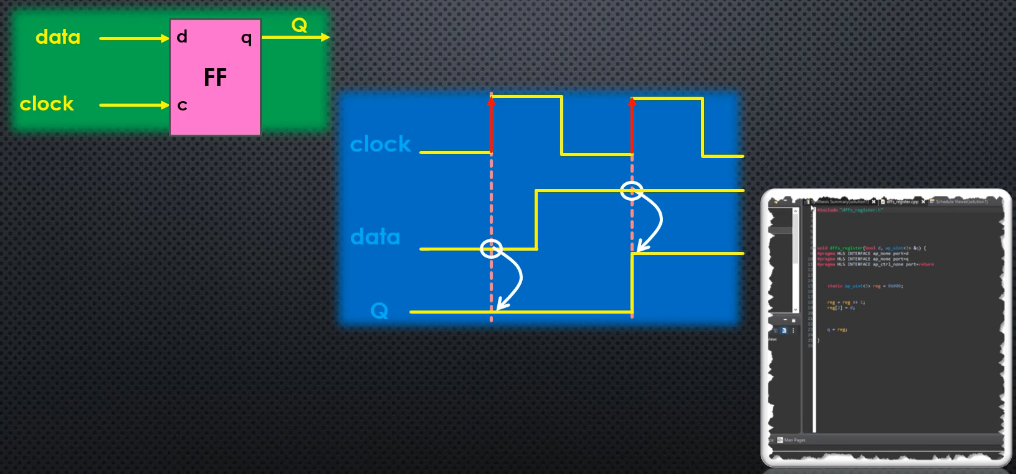
\includegraphics[scale=0.4,frame]{Figures/d_flip_flop/sequential_intro}
\caption{Sequential circuit concepts.}
\label{fig:d_flip_flop:sequential_intro}
\end{figure}


\todo{d flip flop intro} \uti{d flip flop intro:}

\begin{itemize}

\item \textit{To rewrite it later this intro}

\end{itemize}

\newpage
\section{Memory Cell}

As a reminder, sequential circuit contains memory cells which stores some values (in a permanent or temporarily way) when executing some function.\\

The D-FF is the smallest unit that consist these circuit, which can save a 1 bit value.

A simplified version is shown in \autoref{fig:d_flip_flop:d_ff_circuit}.
 
\begin{figure}[h]
\centering
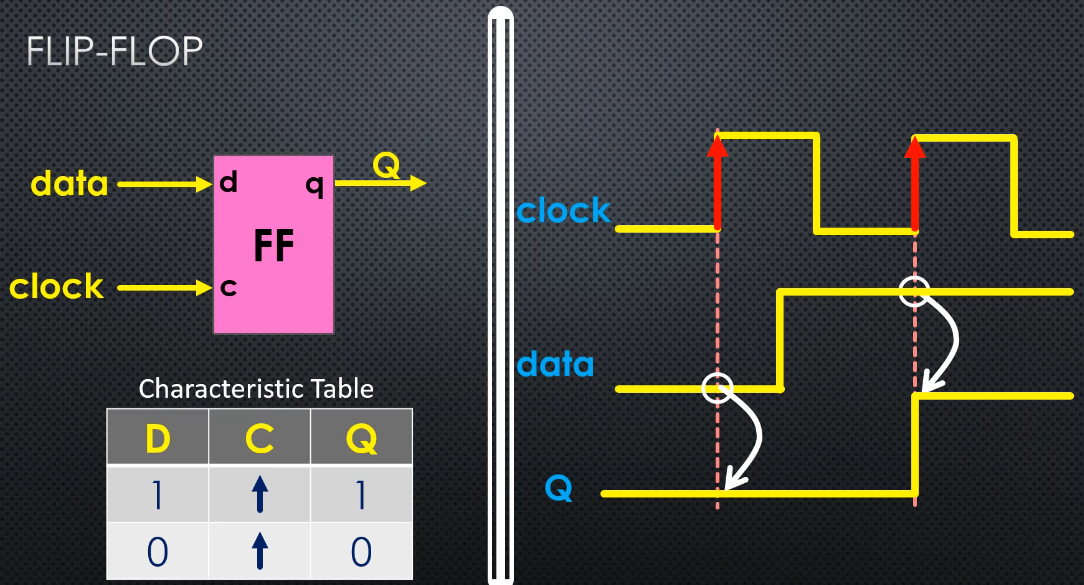
\includegraphics[scale=0.4,frame]{Figures/d_flip_flop/d_ff_circuit}
\caption{Sequential circuit concepts}
\label{fig:d_flip_flop:d_ff_circuit}
\end{figure} 
 
\begin{itemize}

\item It accept 2 input, and generate 1 output. 

\item At each clock cycle, (that is at each rising or falling edge), the flip flop save the data input 

\item This is shown using the table also, where at each rising edge, the data line value at this period is saved at the $Q$ line. 


\end{itemize} 
 
\newpage 

\subsection{Cascaded D-FF}
\label{sub:cascaded_d_ff}

To understand more the D-FF behavior, let's take a cascaded desing shown in  \autoref{fig:d_flip_flop:cascaded_d_ff}.

\begin{figure}[h]
\centering
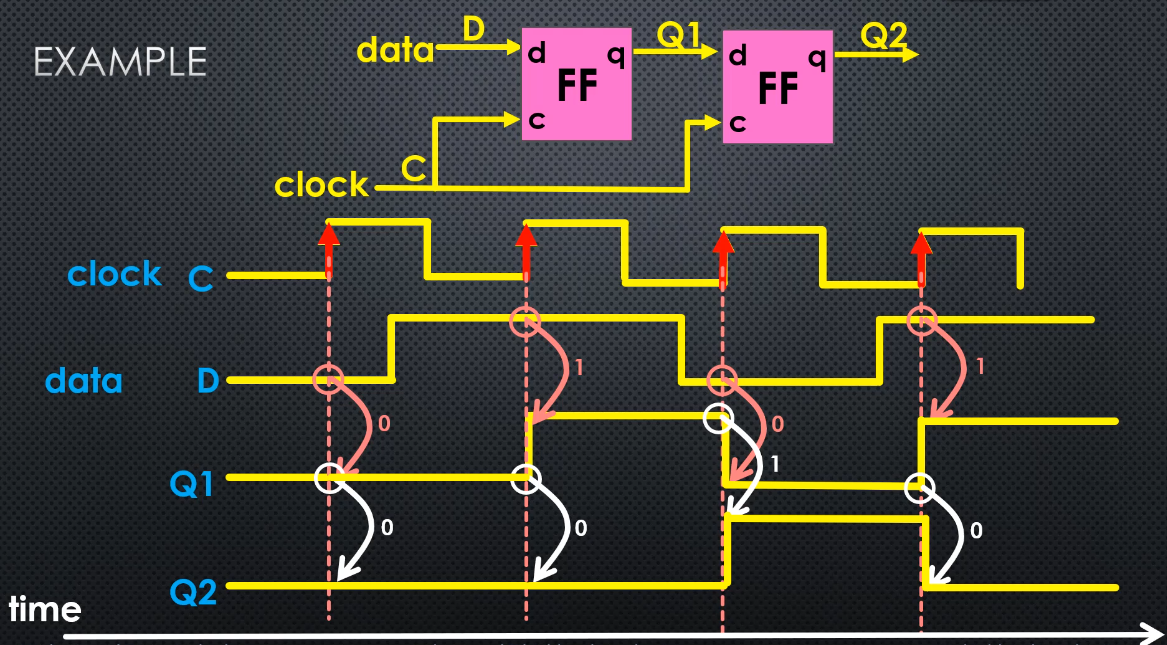
\includegraphics[scale=0.4,frame]{Figures/d_flip_flop/cascaded_d_ff}
\caption{Cascaded D-FF}
\label{fig:d_flip_flop:cascaded_d_ff}
\end{figure}
 
 
\begin{itemize}

\item $\mathrm{1}^\mathrm{st}$ clock cycle: $Q1$ and $Q2$ are both 0

\item $\mathrm{2}^\mathrm{nd}$ clock cycle: $Q1 = 1$ since data line is 1, and $Q2$ still 0 since in $Q1$ was 0 from start of $\mathrm{1}^\mathrm{st}$ till just before $\mathrm{2}^\mathrm{nd}$ clock cycle

\item $\mathrm{3}^\mathrm{rd}$ clock cycle (an important one): $Q1$ is now 0, and $Q2$ changes to 1, \tbi{since the data with respect to $Q2$ is $Q1$}, and $Q1$ in previous clock cycle ($\mathrm{2}^\mathrm{nd}$ rising edge) was 1    

\item $\mathrm{4}^\mathrm{th}$ clock cycle: same concept is applied, $Q1$ will be 1, and $Q2$ changes to 0, since $Q1$ was 0 in the previous clock cycle.

\end{itemize} 


\newpage
\subsection{Quiz} 
 
\underline{Given:} show the output of the following desing shown in \autoref{fig:d_flip_flop:quiz_D_FF_output}.

\begin{figure}[h]
\centering
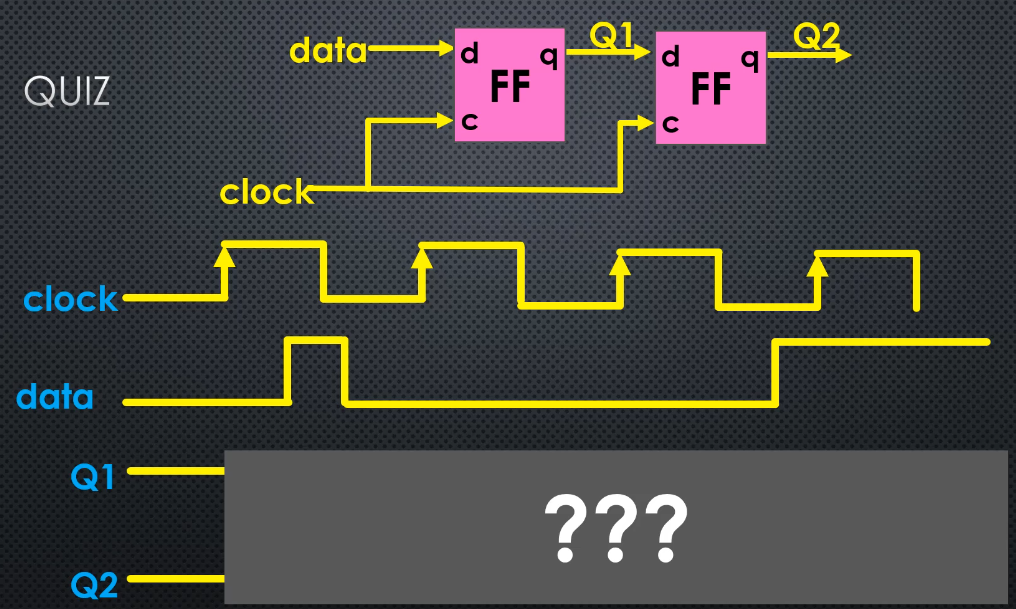
\includegraphics[scale=0.4,frame]{Figures/d_flip_flop/quiz_D_FF_output}
\caption{Given Quiz}
\label{fig:d_flip_flop:quiz_D_FF_output}
\end{figure} 
 
\underline{Solution:} shown in  \autoref{fig:d_flip_flop:quiz_D_FF_output_sol}.
 
\begin{figure}[h]
\centering
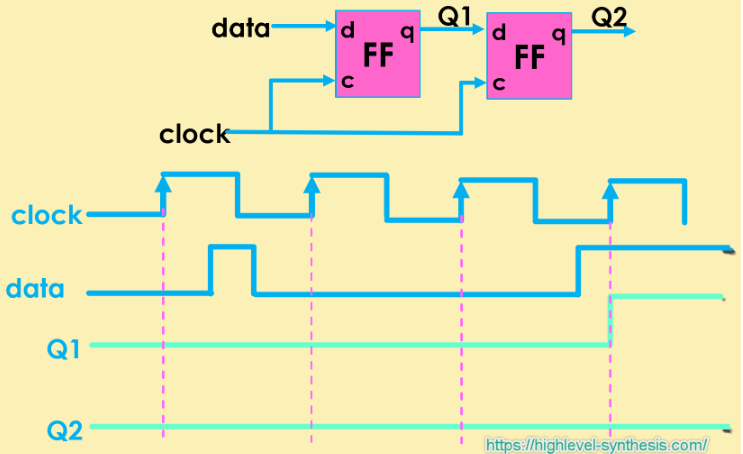
\includegraphics[scale=0.4,frame]{Figures/d_flip_flop/quiz_D_FF_output_sol}
\caption{Quiz solution}
\label{fig:d_flip_flop:quiz_D_FF_output_sol}
\end{figure}


\newpage
\section{Sequential Circuit}

Sequential circuit are circuit which uses input from previous states, so they need some systems to store or transfer input values, and memory cells are perfect candidates for that.

A general block diagram of a sequential circuit is shown in \autoref{fig:d_flip_flop:seq_circuit_block}.  

\begin{figure}[h]
\centering
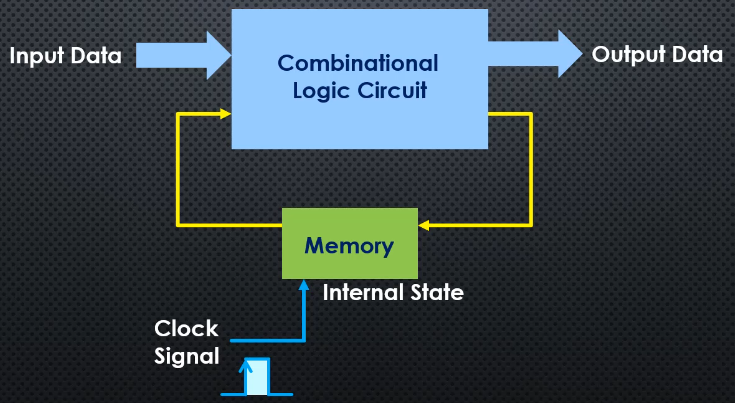
\includegraphics[scale=0.4,frame]{Figures/d_flip_flop/seq_circuit_block}
\caption{Sequential circuit blocks}
\label{fig:d_flip_flop:seq_circuit_block}
\end{figure}

It is composed from 2 parts: 

\begin{itemize}

\item a combinational one that perform the logic functions

\item a memory part that stores the state execution part, and transfer the data between the sequences.

\end{itemize}

The clock signal determines the boundries of execution between sequences.\\

\autoref{fig:d_flip_flop:seq_circuit_block} is general to represent all sequential circuits. The block shown in \autoref{fig:d_flip_flop:seq_circuit_block_2} is a more special, because the memory part takes directly input and generate directly some output.

\begin{figure}[h]
\centering
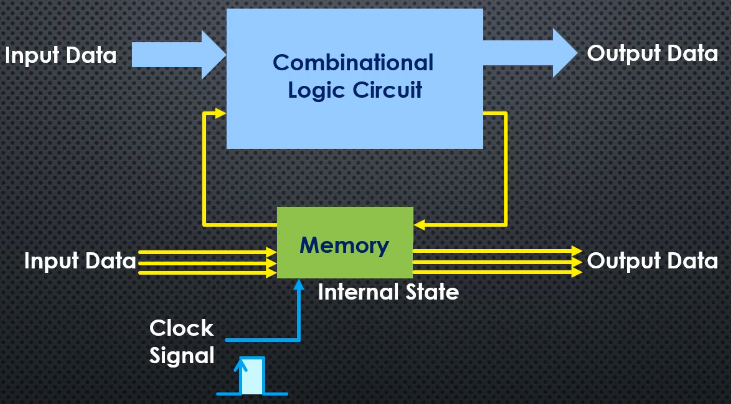
\includegraphics[scale=0.4,frame]{Figures/d_flip_flop/seq_circuit_block_2}
\caption{Sequential circuit: input and output are passed to memory cell directly}
\label{fig:d_flip_flop:seq_circuit_block_2}
\end{figure}

\subsection{Tracking a sequential circuit}
\label{sub:track_seq_circuit}

Let's take an example to understand how a sequential circuit is executed. The example is shown in \autoref{fig:d_flip_flop:ex_tracking}.

\begin{figure}[h]
\centering
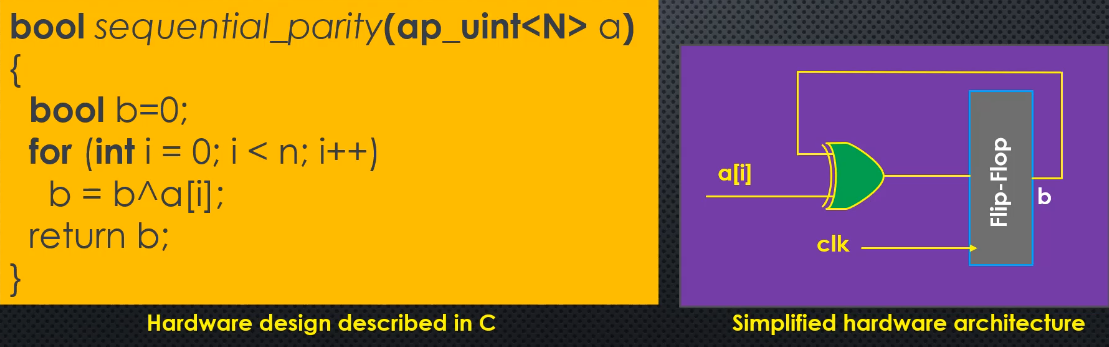
\includegraphics[scale=0.4,frame]{Figures/d_flip_flop/ex_tracking}
\caption{Parity bit example}
\label{fig:d_flip_flop:ex_tracking}
\end{figure}

The loop is kept, that is it is not unrolled, so the circuit is sequential.

The D-FF is used at the output to store the result, and use it in the next iteration. However, if we pay attention, the operation \verb|b = b^a[i]| consist of 3 operation: reading \verb|b| value, computing the result, and save the result. This is shown in \autoref{fig:d_flip_flop:ex_tracking_one_iter}.


\begin{figure}[h]
\centering
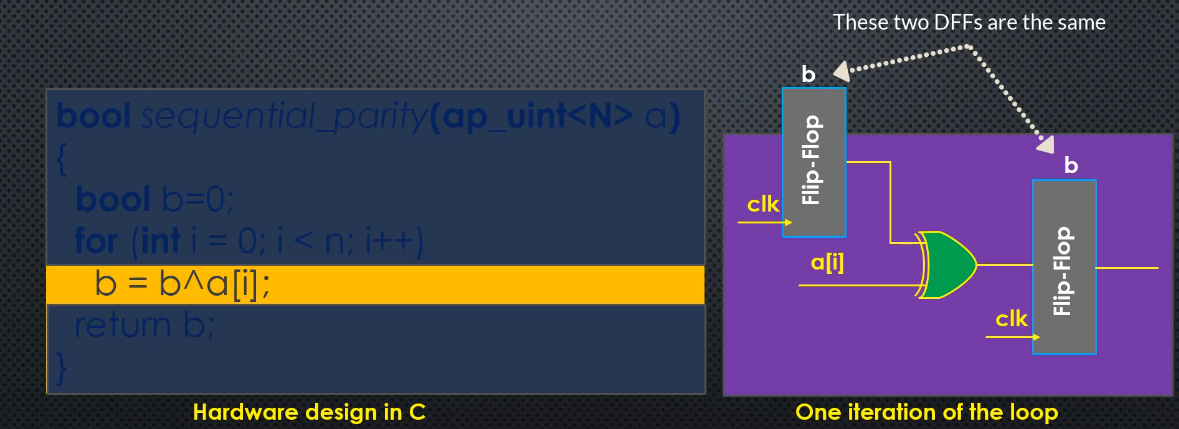
\includegraphics[scale=0.4,frame]{Figures/d_flip_flop/ex_tracking_one_iter}
\caption{Parity bit for 1 iteration}
\label{fig:d_flip_flop:ex_tracking_one_iter}
\end{figure}

\underline{Note:} the \verb|a| variable is given directly throughout the function, and doesn't need to be stored. It can be implemented as a set of wires.\\

\newpage
Now let's generalize the concept from 1 iteration to many iterations, as shown in \autoref{fig:d_flip_flop:ex_tracking_all_iter}.


\begin{figure}[h]
\centering
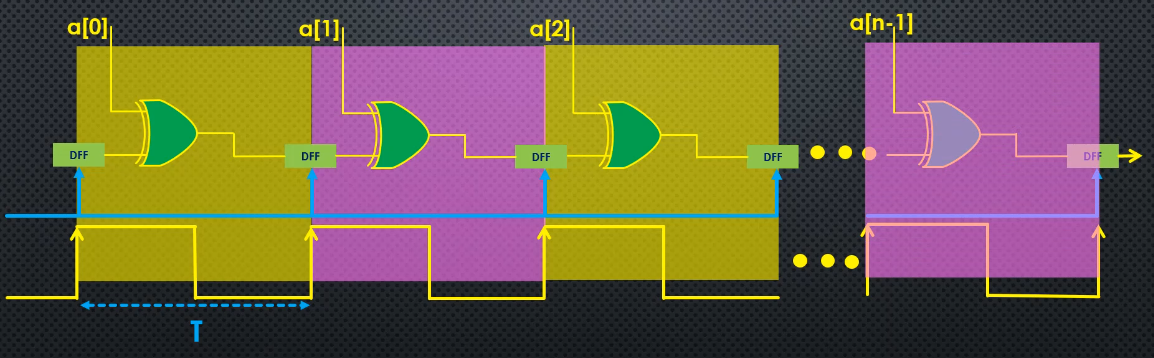
\includegraphics[scale=0.4,frame]{Figures/d_flip_flop/ex_tracking_all_iter}
\caption{Parity bit for 1 iteration}
\label{fig:d_flip_flop:ex_tracking_all_iter}
\end{figure}

\begin{itemize}

\item It is assumed that the loop body is performed under 1 clock cycle, denoted by $T$.

\item At each clock period, the circuit read the \verb|b| value, perform the logic function (which is a \verb|XOR|), then save the computed value in the same memory

\item Same operation is repeated at each clock cycle

\end{itemize}

The general concept of circuit execution is shown in \autoref{fig:d_flip_flop:sequential_circuit_execution}.

\begin{figure}[h]
\centering
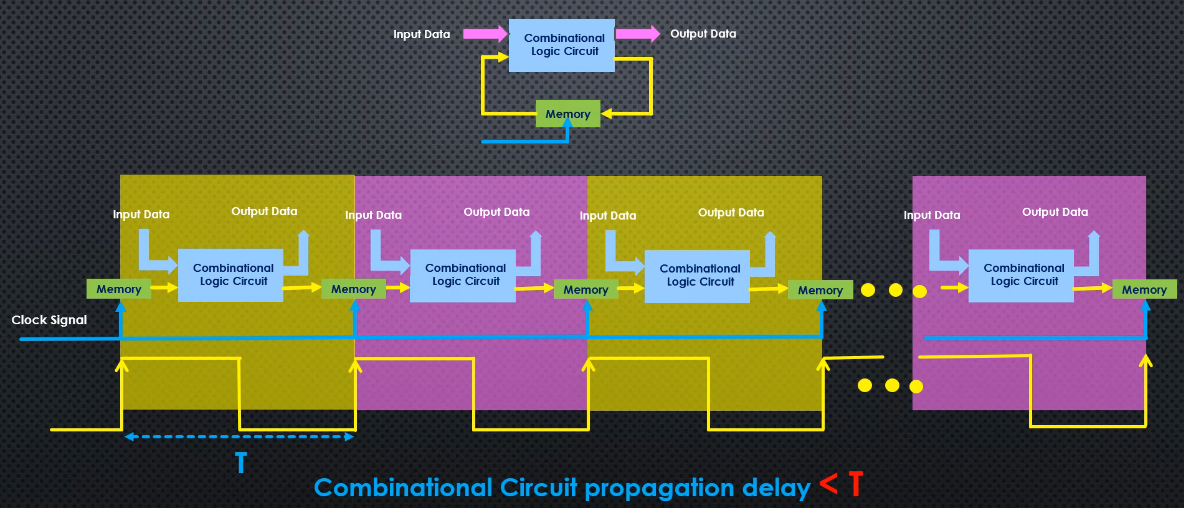
\includegraphics[scale=0.4,frame]{Figures/d_flip_flop/sequential_circuit_execution}
\caption{General execution of sequential circuit}
\label{fig:d_flip_flop:sequential_circuit_execution}
\end{figure}

\newpage
\section{Clock Signal}

Clock signals plays an important role in digital system, as seen in \ref{sub:circuit_types}, where comparison with $t_p$ defines the nature of circuit (sequential or combinational). In this section we move in more detail about the clock signal.

\subsection{Setup and hold time}
\label{sub:setup_hold_time}

Let's consider a D-FF. We know that a D-FF saves the values before the rising edge.

\begin{figure}[h]
\centering
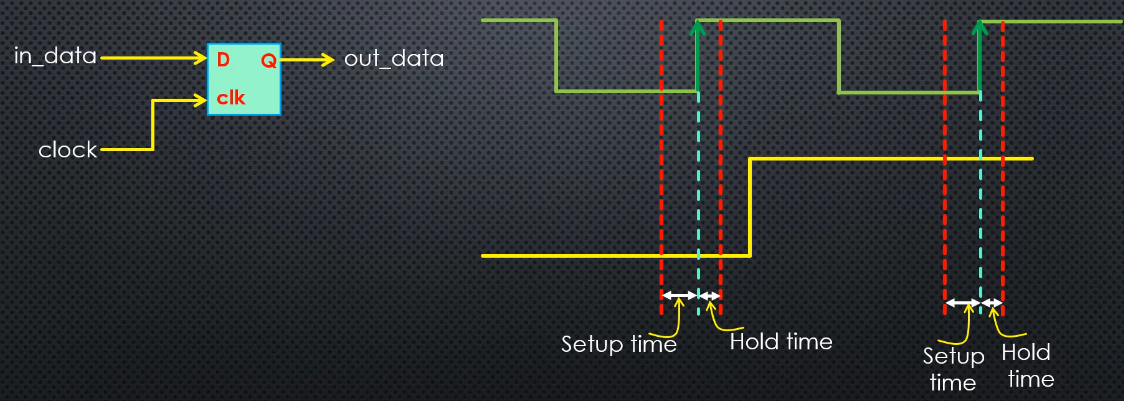
\includegraphics[scale=0.4,frame]{Figures/d_flip_flop/setup_hold_time}
\caption{Setup and hold time for a clock signal}
\label{fig:d_flip_flop:setup_hold_time}
\end{figure}

\begin{itemize}

\item  At the rising edge, we have 2 intervals, before and after in which the values need to be stable.

	\begin{itemize}
	\item These time intervals are \textit{setup} (before) and \textit{hold}(after). During this interval, the D-FF sample the value and save its state. 
	\end{itemize}

\item The duration of these interval is due to the underlying technolgies related to the fabrication of the FPGA, thus their values are constant and can't be changed during the desing

\item The combionational circuit providng D-FF input (recall and see \autoref{fig:d_flip_flop:seq_circuit_block}) should give input before these interval, and keep the value unchanged during sampling time.

\end{itemize}

\newpage
\subsection{$t_p$, setup and hold time}
\label{sub:tp_setup_hold_time}

Consider the simple sequential circuit shwon in \autoref{fig:d_flip_flop:tp_setup_hold_time}.

\begin{figure}[h]
\centering
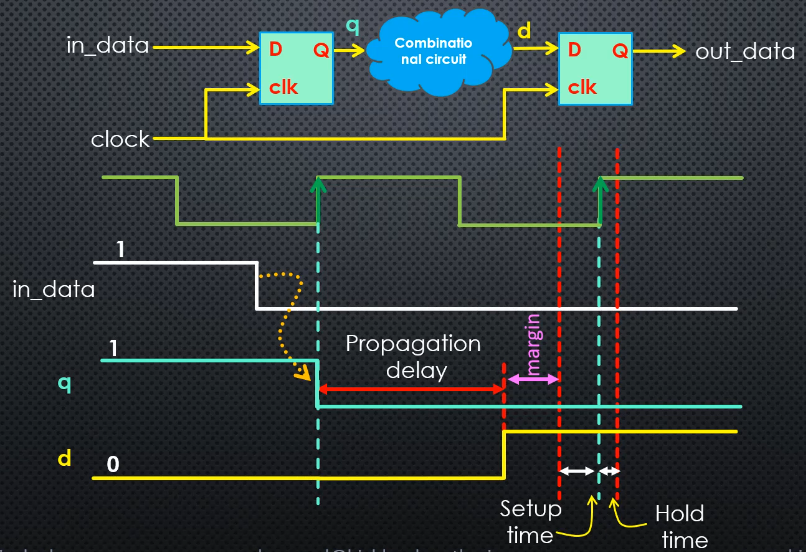
\includegraphics[scale=0.4,frame]{Figures/d_flip_flop/tp_setup_hold_time}
\caption{Propagation delay with setup and hold time}
\label{fig:d_flip_flop:tp_setup_hold_time}
\end{figure}

\underline{Note:} notice that between the 2 D-FF, there is a combinational circuit in between, so it is different than the cascaded desing seen in \ref{sub:cascaded_d_ff}.

\begin{itemize}

\item  Initially, \verb|in-data| value is 1, then before the $\mathrm{1}^\mathrm{st}$ rising edge, it changes its value to 0

\item Thus, \verb|q| (output of $\mathrm{1}^\mathrm{st}$ D-FF) is now 0

\item The combinational circuit takes \verb|q| as input, and after some $t_p$, the output \verb|d| changes from 0 $\rightarrow$ 1

\item Then $\mathrm{2}^\mathrm{nd}$ D-FF saves the value of the \verb|d| value at the $\mathrm{2}^\mathrm{nd}$ rising edge, \tbi{if we respect the condition of setup and hold time}

\end{itemize}

Notice that between $t_p$ and setup time there is some margin, and it is called \textit{slack time}, and desingners prefer to have such margin due to relaibility and uncertainty.\\

\uti{margin and slack time:} \todo{margin and slack time}

\begin{itemize}

\item \textit{To see later why a margin is preferred, to do some research about it}

\end{itemize}


\newpage
\section{Circuit State}
\label{sec:circuit_state}

We seen before that clock signal gives the order to save new value, and transfer this value to the next state of the circuit.

In this section we explore in details the concept of a state, and what does it means exactly.\\

Sequential circuit, and unilike combinational one depdens also at \textit{past input and outputs}. FF are used to save (keep track) values of past input and output at each clock cycle.

The values stored in the FF at each clock cycle is called \textit{state of the sequential circuit}. In other words, a state $s_n$ encapsulate past input and output \textit{up to a specific time}. Therefore, \textit{the transition between states} can \textit{describe the behaviour of a sequential circuit}.	

\begin{figure}[h]
\centering
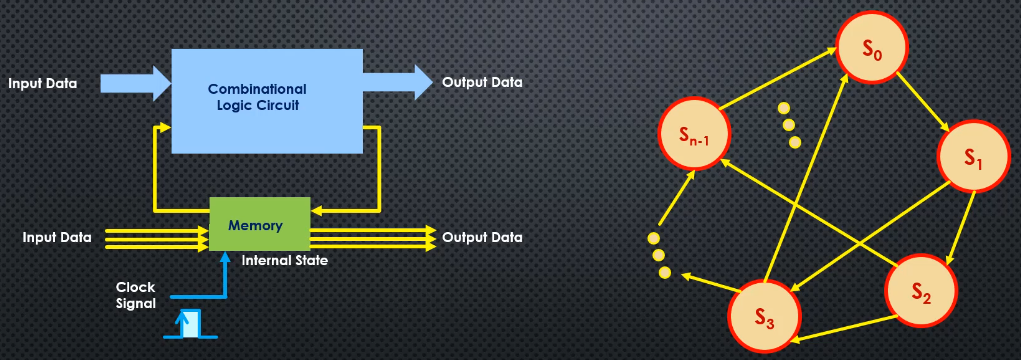
\includegraphics[scale=0.4,frame]{Figures/d_flip_flop/circuit_state}
\caption{Sequential circuit state $s_n$}
\label{fig:d_flip_flop:circuit_state}
\end{figure}

Later, we see how we can use a FSM to represent the transition model of states, and describe a wide range of sequential circuit.

\subsection{D-FF State}

Let's understand more the concept of state by taking a D-FF as example. The state diagram is shown in \autoref{fig:d_flip_flop:d_ff_state}.

\begin{figure}[h]
\centering
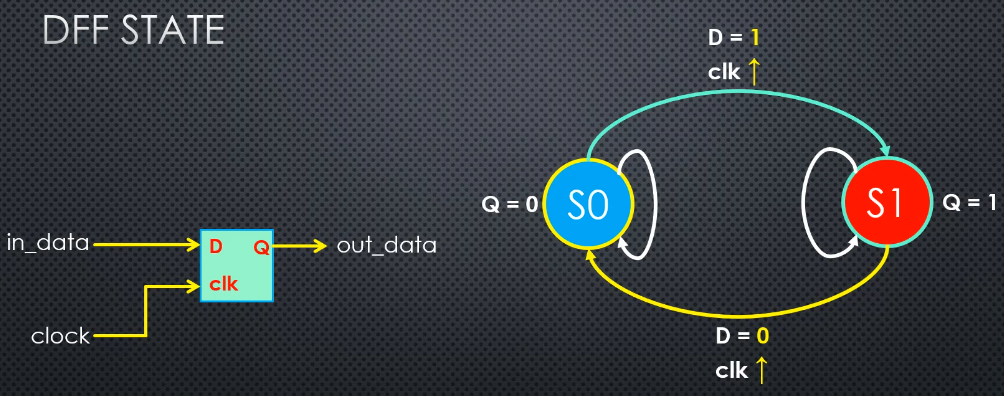
\includegraphics[scale=0.4,frame]{Figures/d_flip_flop/d_ff_state}
\caption{D-FF state diagram}
\label{fig:d_flip_flop:d_ff_state}
\end{figure}

\begin{itemize}

\item A D-FF can have 2 states $s_0$ and $s_1$ since it has only 2 output: 1 or 0.

\item It transition from $s_0 \, \rightarrow \, s_1$ if $D \, = \, 1$ at the rising edge of the clock

\item It transition from $s_1 \, \rightarrow \, s_0$ if $D \, = \, 0$ at the rising edge of the clock

\item Also, $s_0$ loop at itself if $D \, = \, 0$

\item Same for $s_1$ if $D \, = \, 1$ 

\end{itemize}

\subsection{Some state diagram rules}

Now we note some state diagram rules we should keep in mind

\begin{figure}[h]
\centering
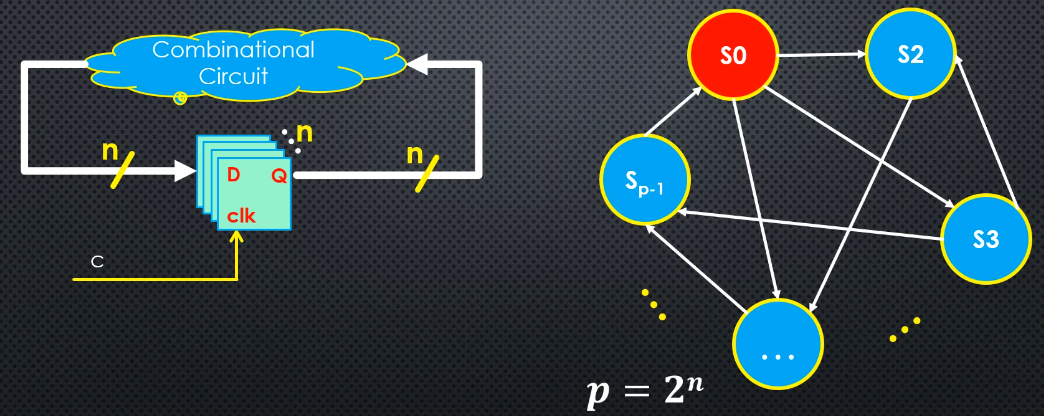
\includegraphics[scale=0.4,frame]{Figures/d_flip_flop/state_rules}
\caption{State diagram rules}
\label{fig:d_flip_flop:state_rules}
\end{figure}

\begin{itemize}

\item A circuit having $n$ memory cells can have $p$ states, where $p \, = \, 2^n$ is the maximum

\item Each state diagram should have a \textit{starte state} $s_0$ from which the state diagram starts

	\begin{itemize}
	\item We should also have a least 1 path from each $s_n$ state to the starter state $s_0$ in order to reset the circuit
	
	\item a reset signal in a sequential circuit is responsible to putting the circuit in some known state
	
	\end{itemize}

\end{itemize}

\newpage
\subsection{Quiz}

\underline{Given:} Draw the state diagram of the circuit shown in \autoref{fig:d_flip_flop:quiz_state_diagram}.

\begin{figure}[h]
\centering
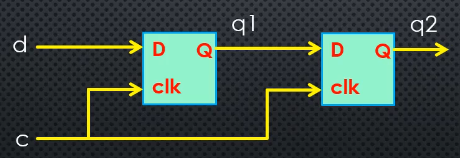
\includegraphics[scale=0.4,frame]{Figures/d_flip_flop/quiz_state_diagram}
\caption{Quiz state diagram}
\label{fig:d_flip_flop:quiz_state_diagram}
\end{figure}

\underline{Solution:} solution is shown in \autoref{quiz_state_diagram_sol}.

\begin{figure}[h]
\centering
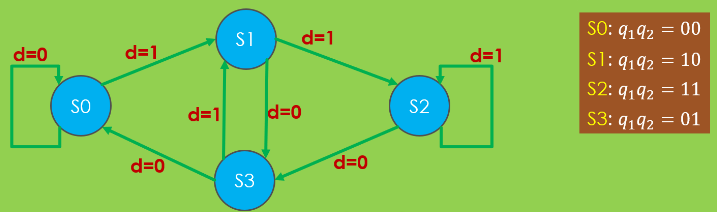
\includegraphics[scale=0.4,frame]{Figures/d_flip_flop/quiz_state_diagram_sol}
\caption{Quiz state diagram solution}
\label{fig:d_flip_flop:quiz_state_diagram_sol}
\end{figure}

\todo{quiz state diagram} \uti{quiz state diagram:}

\begin{itemize}

\item \textit{to rewrite a better explanation later when doing exercices and finishing the chapter}

\end{itemize}

\newpage
\section{Reset Signal}

Sequential circuits follows a series of events (states), so from a desing point of view their should be a mechanism that should put the circuit in a start or a at least a known state. This mechanism is known as the reset signal.\\

Let's consider a reset signal in case of a D-FF as shown in \autoref{fig:d_flip_flop:reset_sig_d_ff}.

\begin{figure}[h]
\centering
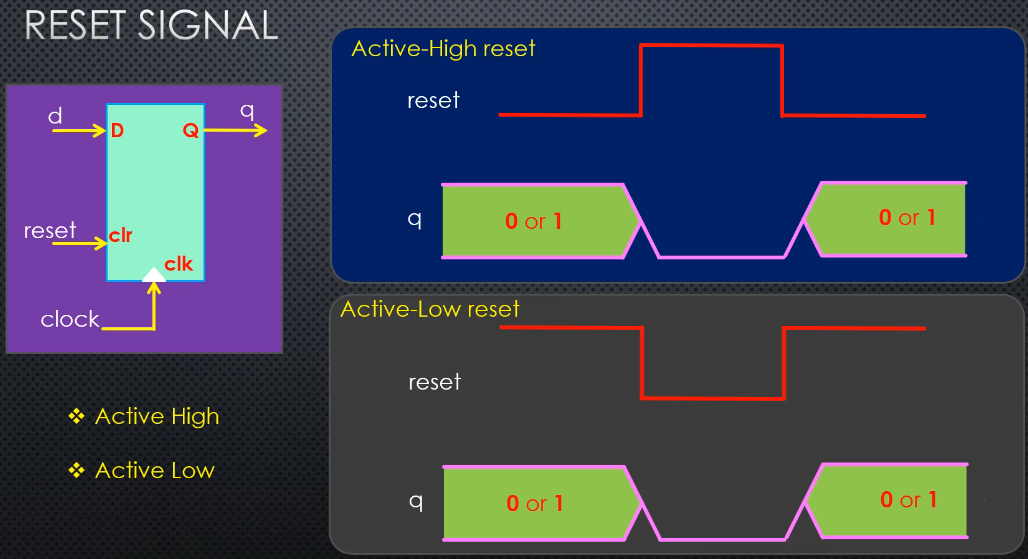
\includegraphics[scale=0.4,frame]{Figures/d_flip_flop/reset_sig_d_ff}
\caption{Reset signal}
\label{fig:d_flip_flop:reset_sig_d_ff}
\end{figure}

\begin{itemize}

\item A reset signal should set the output $q$ to 0, whatever there is at the data line (the input side)

\item It can be active low or active high

\item We can see in \autoref{fig:d_flip_flop:reset_sig_d_ff}, that as long as the reset signal is ON (active low or high), $q$ value is always 0

\end{itemize}

\subsection{Async vs sync Reset}

There are 2 types of reset for the signal:

\begin{itemize}

\item synchronous: the devices wait the for the next edge of the clock

\item asynchronous: the signal doesn't depends at the clock 

\end{itemize}

\newpage
\autoref{fig:d_flip_flop:async_sync_reset} shows an example for the 2 reset type, where the reset signal is active high.

\begin{figure}[h]
\centering
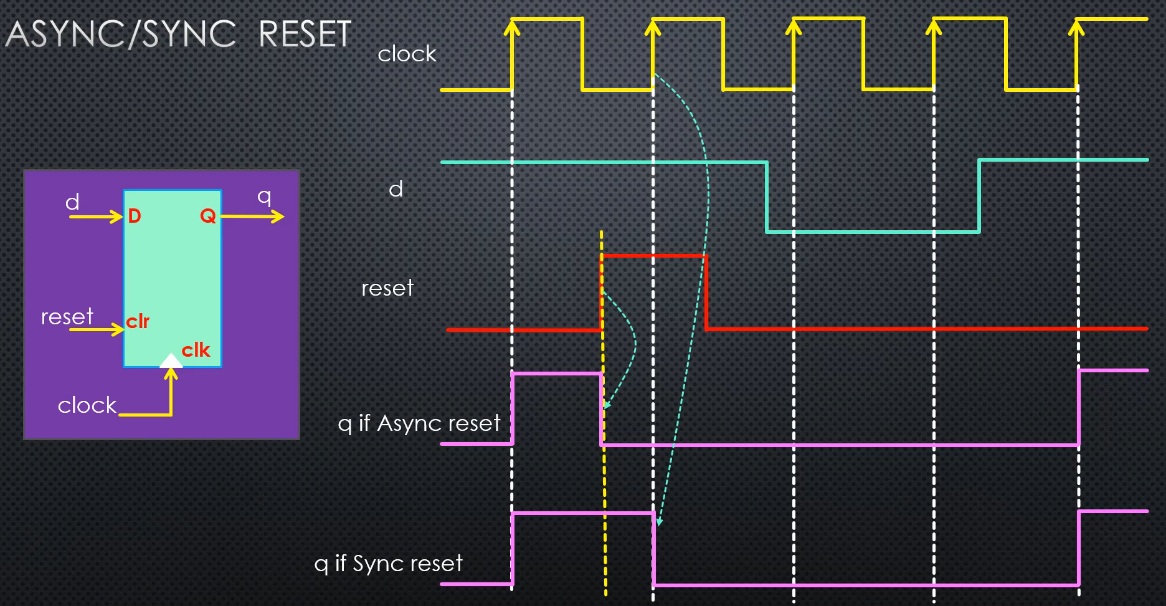
\includegraphics[scale=0.4,frame]{Figures/d_flip_flop/async_sync_reset}
\caption{Asynchrounous and synchronous reset}
\label{fig:d_flip_flop:async_sync_reset}
\end{figure}

\begin{itemize}

\item Notice in asynchrnous case, the $q$ output directly switch to 0 and is not affected by the clock

\item Whereas in synchronous case, $q$ wait for the next clock cycle to swith to 0

\item Once the reset signal is low (disappear), the D-FF continue to acte normally, and sample data at each rising edge of the clock

\end{itemize}


\newpage
\subsection{Reset configuration in HLS}

\autoref{fig:d_flip_flop:reset_conf_hls} shows the different configuration we can make using \verb|Vitis|.

\begin{figure}[h]
\centering
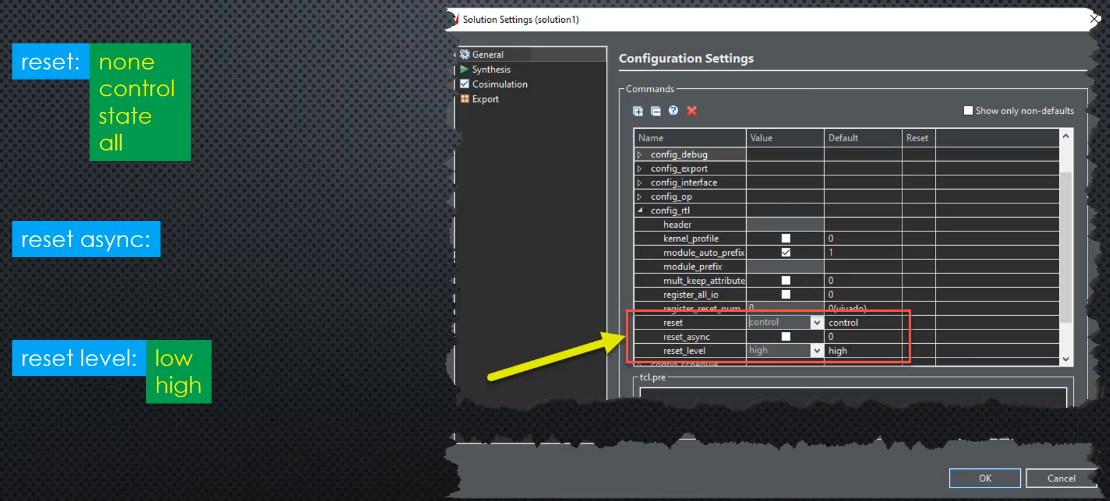
\includegraphics[scale=0.4,frame]{Figures/d_flip_flop/reset_conf_hls}
\caption{Asynchrounous and synchronous reset}
\label{fig:d_flip_flop:reset_conf_hls}
\end{figure}

\uti{Reset config} \uti{Reset config:}

\begin{itemize}

\item \textit{Source: section 3, video 13}

\item \textit{I didn't understand fully the options of the reset part}

\item \textit{To return to them later, when explaining them in some next chapters}

\end{itemize}


\newpage
\subsection{Quiz}

\underline{Given:} consider the circuit shown in \autoref{fig:d_flip_flop:quiz_reset}. Find the the output value $q_1$ and $q_2$.

\begin{figure}[h]
\centering
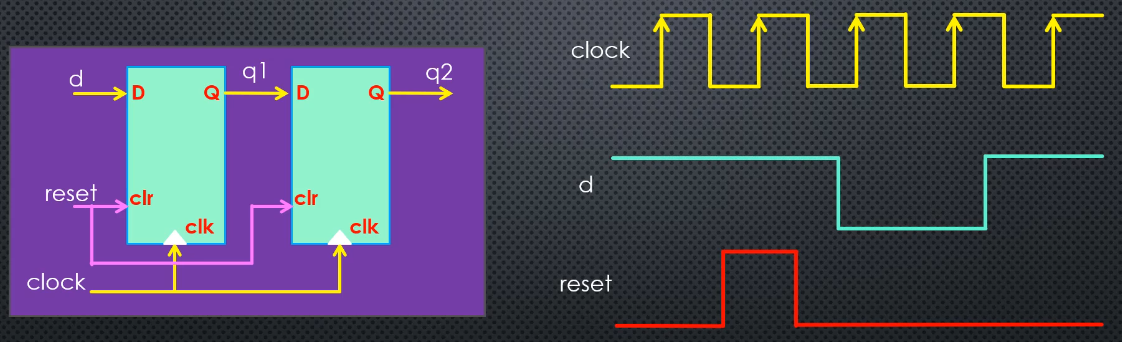
\includegraphics[scale=0.4,frame]{Figures/d_flip_flop/quiz_reset}
\caption{Quiz reset}
\label{fig:d_flip_flop:quiz_reset}
\end{figure}

\underline{Solution:} shown in \autoref{fig:d_flip_flop:quiz_reset_sol}.

\begin{figure}[h]
\centering
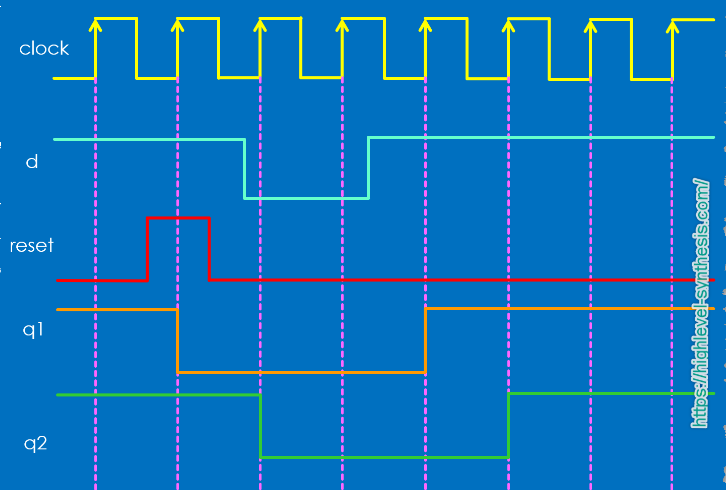
\includegraphics[scale=0.4,frame]{Figures/d_flip_flop/quiz_reset_sol}
\caption{Quiz reset}
\label{fig:d_flip_flop:quiz_reset_sol}
\end{figure}


\todo{quiz reset} \uti{quiz reset}

\begin{itemize}

\item \textit{To get back to it later when practicing}

\end{itemize}

\newpage
\section{Registers}

This section contains a refresher about registers, as we don't nee to dive into details into registers in \verb|HLS| like classical digital desing.

A register, which is another type of sequential circuit, is simply a series of D-FF with the same control mechanism, that is they have the same reset and clock, so we can write and read from them all at the same time.

\begin{figure}[h]
\centering
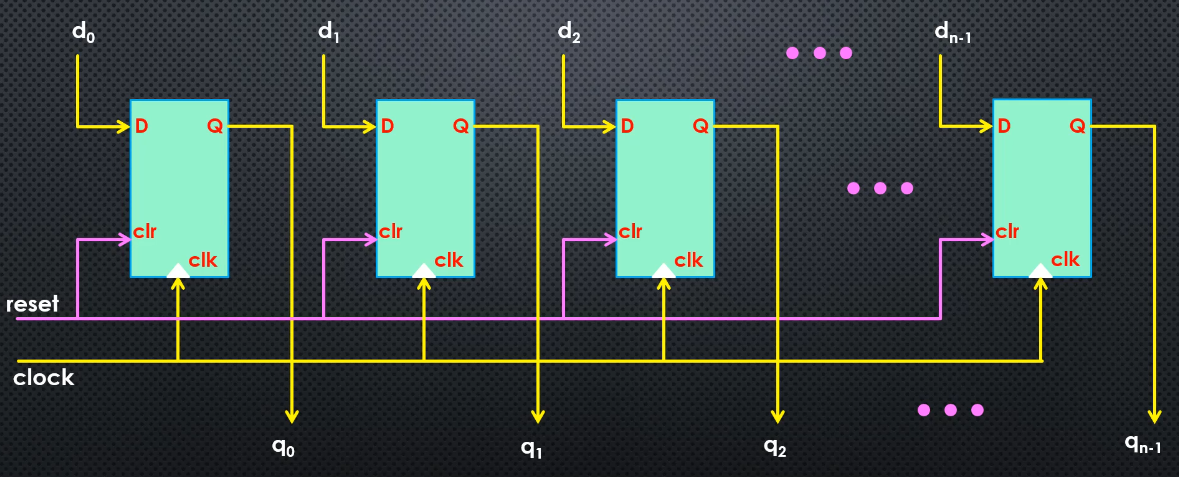
\includegraphics[scale=0.4,frame]{Figures/d_flip_flop/register}
\caption{Register}
\label{fig:d_flip_flop:register}
\end{figure}

There are many types of registers like shift register and parallel load register shown in \autoref{fig:d_flip_flop:register_types}.

\begin{figure}[h]
\centering
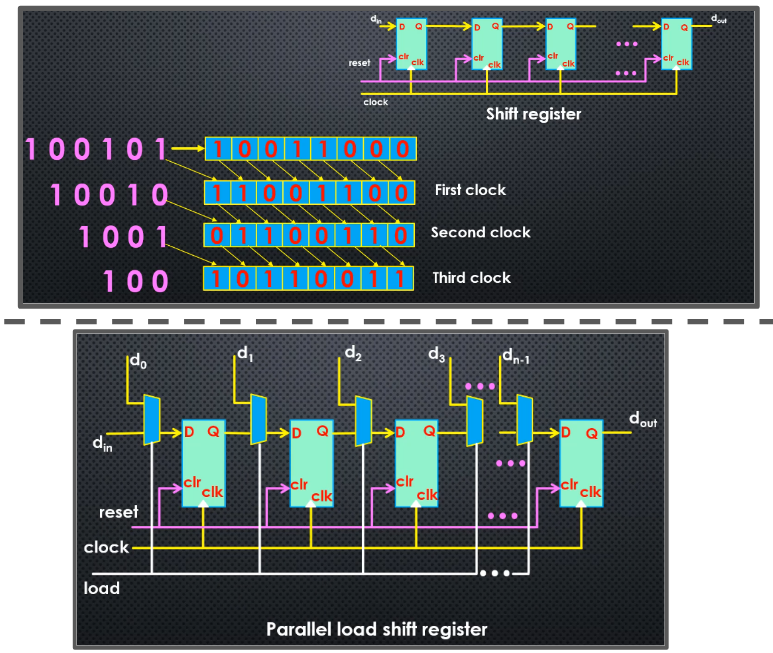
\includegraphics[scale=0.4,frame]{Figures/d_flip_flop/register_types}
\caption{Register}
\label{fig:d_flip_flop:register_types}
\end{figure}

\newpage
In \verb|HLS|, a static variable is mapped to a register, and the register type depends on the type of manipulation we are doing to this static variable. An example is shown in \autoref{fig:d_flip_flop:reg_hls}.

\begin{figure}[h]
\centering
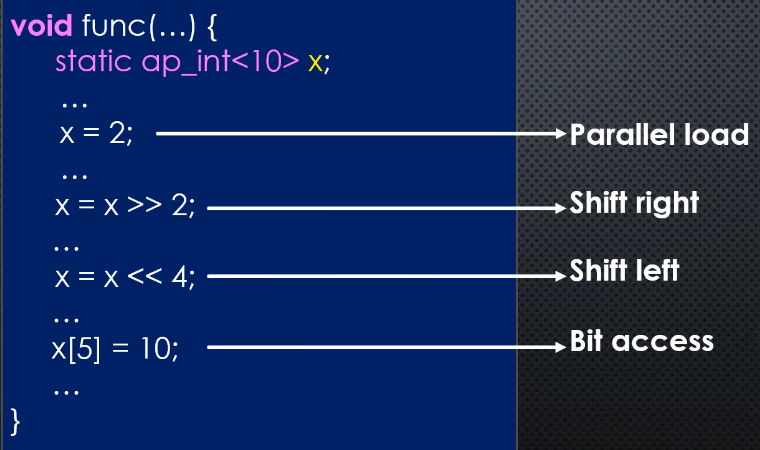
\includegraphics[scale=0.4,frame]{Figures/d_flip_flop/reg_hls}
\caption{Register in HLS}
\label{fig:d_flip_flop:reg_hls}
\end{figure}

\subsection{Quiz}

\underline{Given:} How many register hardware we expect to see in the code shown in 
\autoref{fig:d_flip_flop:quiz_reg}

\begin{figure}[h]
\centering
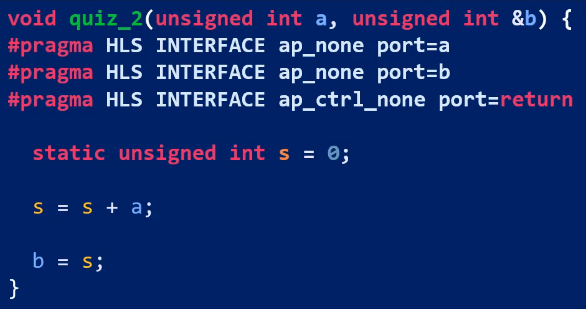
\includegraphics[scale=0.4,frame]{Figures/d_flip_flop/quiz_reg}
\caption{Quiz given}
\label{fig:d_flip_flop:quiz_reg}
\end{figure}

\underline{Solution:} see \verb|DFF-Register-Quiz-Solution.pdf|.\\

\todo{quiz reg} \uti{quiz reg:} \textit{To redo this exercice later}.





%=============================================
%=============================================
%=============================================

\newpage
\section{Summary D-FF}

\begin{itemize}

\item Sequential circuit: systems which depends on present \textit{and past input and output}

	\begin{itemize}
	\item They use FF to keep track and save past input and outputs at each clock cycle
	\end{itemize}

\item Fundamental unit in sequential circuit: D-FF which saves value at clock edges (rising or falling)

	\begin{itemize}
	\item \ref{sub:cascaded_d_ff} important explanation about cascaded of D-FF, and how the $\mathrm{2}^\mathrm{nd}$ D-FF reacts
	
	\item this should kept in mind
	\end{itemize}

\item Clock signal functionality

	\begin{itemize}
	
	\item Combinational functions are executed (\ref{sub:track_seq_circuit} for the parity bit example)	
	
	\item between their boundaries, values are saved and transferred to new state
	
	\end{itemize}


\item Paramter of clock signal:

	\begin{itemize}

	\item setup and hold time (\ref{sub:setup_hold_time})

	\item $t_p$
	
	\item uncertainty, and usually in tools such as \verb|Vitis|, it is configured as precentage of clock period.
	\end{itemize}

\item D-FF saves values just before rising edge (or falling edge, depends on which edge), such that it respects the clock constraint coniditons (\ref{sub:tp_setup_hold_time})

	\begin{itemize}
	\item $\leftrightarrow$ input should provided before setup and hold time
	
	\item input value shoud be constant during this period
	\end{itemize}


\item State diagram informations (\ref{sec:circuit_state})

	\begin{itemize}
	\item number of states equal to the number of output logic values we can have
	
	\item A transition from 1 state to another occurs whnen an input change, or at some clock cycle (like a state looping at itself)
	
	\item we should have a starter state $s_0$ from which system start to perform its task
	
	\item we should have 1 path from each state to $s_0$ so we could have a reset signal
	
	\item Number of states $p$ equal at most $2^n$, where $n$ is number of logic cells (FF)
	
	
	\item Beaware that $p$ is not the same as the number of transitions (number of edges)
	\end{itemize}

\end{itemize}















 